\documentclass[tikz,border=5mm]{standalone}
\usepackage{amsmath}
\usetikzlibrary{patterns}

\begin{document}
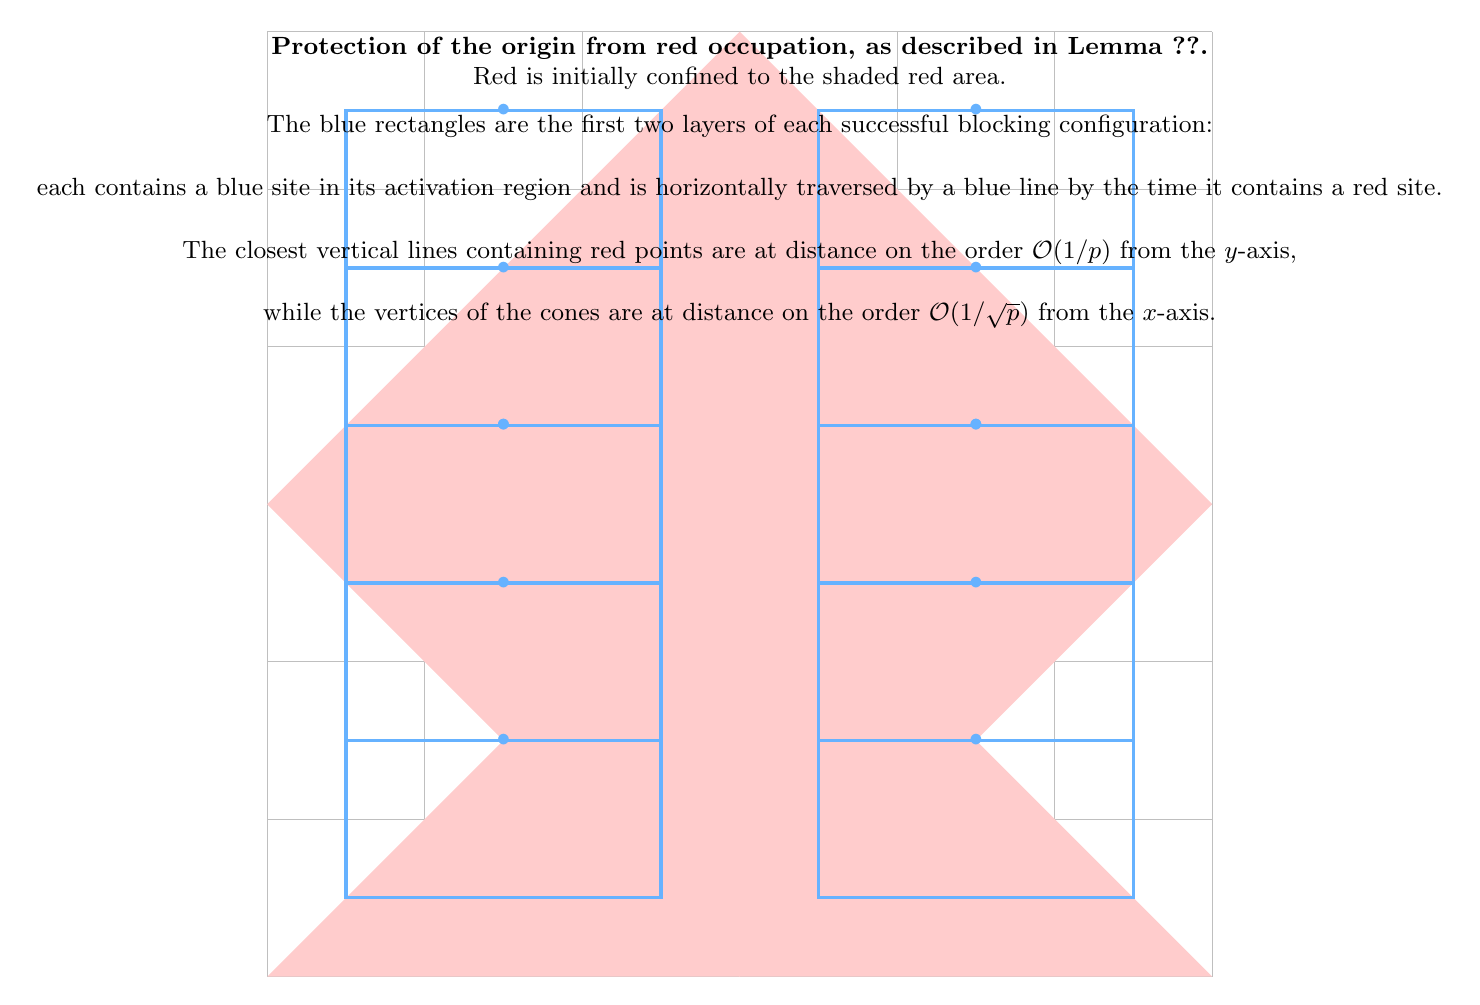
\begin{tikzpicture}[scale=2]

% Define colors
\definecolor{myred}{RGB}{255, 153, 153} % Light pink/red shade
\definecolor{myblue}{RGB}{102, 178, 255} % Light blue shade

% Draw the grid lines
\draw[gray!50] (-3,-3) grid (3,3);

% Draw the red-shaded areas (cones)
\fill[myred!50] (-3,0) -- (0,3) -- (0,-3) -- cycle;
\fill[myred!50] (0,3) -- (3,0) -- (0,0) -- cycle;
\fill[myred!50] (0,0) -- (3,-3) -- (-3,-3) -- cycle;
\fill[myred!50] (-3,0) -- (0,-3) -- (3,0) -- cycle;

% Draw the blue rectangles and horizontal lines
% Top-left quadrant
\draw[myblue, very thick] (-2.5,2.5) rectangle (-0.5,1.5);
\draw[myblue, very thick] (-2.5,1.5) rectangle (-0.5,0.5);
\draw[myblue, very thick] (-2.5,0.5) rectangle (-0.5,-0.5);
\foreach \y in {2,1,0} {
    \draw[myblue, very thick] (-2.5,\y+0.5) -- (-0.5,\y+0.5);
    \node[myblue] at (-1.5,\y+0.5) {$\bullet$};
}

% Top-right quadrant
\draw[myblue, very thick] (0.5,2.5) rectangle (2.5,1.5);
\draw[myblue, very thick] (0.5,1.5) rectangle (2.5,0.5);
\draw[myblue, very thick] (0.5,0.5) rectangle (2.5,-0.5);
\foreach \y in {2,1,0} {
    \draw[myblue, very thick] (0.5,\y+0.5) -- (2.5,\y+0.5);
    \node[myblue] at (1.5,\y+0.5) {$\bullet$};
}

% Bottom-left quadrant
\draw[myblue, very thick] (-2.5,-2.5) rectangle (-0.5,-1.5);
\draw[myblue, very thick] (-2.5,-1.5) rectangle (-0.5,-0.5);
\draw[myblue, very thick] (-2.5,-0.5) rectangle (-0.5,0.5);
\foreach \y in {-2,-1,0} {
    \draw[myblue, very thick] (-2.5,\y+0.5) -- (-0.5,\y+0.5);
    \node[myblue] at (-1.5,\y+0.5) {$\bullet$};
}

% Bottom-right quadrant
\draw[myblue, very thick] (0.5,-2.5) rectangle (2.5,-1.5);
\draw[myblue, very thick] (0.5,-1.5) rectangle (2.5,-0.5);
\draw[myblue, very thick] (0.5,-0.5) rectangle (2.5,0.5);
\foreach \y in {-2,-1,0} {
    \draw[myblue, very thick] (0.5,\y+0.5) -- (2.5,\y+0.5);
    \node[myblue] at (1.5,\y+0.5) {$\bullet$};
}

% Add annotations
\node[align=center, font=\small] at (0,2.8) {\textbf{Protection of the origin from red occupation, as described in Lemma~\ref{protection lemma}.}\\ Red is initially confined to the shaded red area.};
\node[align=center, font=\small] at (0,2.4) {The blue rectangles are the first two layers of each successful blocking configuration:};
\node[align=center, font=\small] at (0,2.0) {each contains a blue site in its activation region and is horizontally traversed by a blue line by the time it contains a red site.};
\node[align=center, font=\small] at (0,1.6) {The closest vertical lines containing red points are at distance on the order $\mathcal{O}(1/p)$ from the $y$-axis,};
\node[align=center, font=\small] at (0,1.2) {while the vertices of the cones are at distance on the order $\mathcal{O}(1/\sqrt{p})$ from the $x$-axis.};

\end{tikzpicture}
\end{document}